\documentclass{article}

\usepackage{amsmath}
\usepackage{amssymb}
\usepackage{geometry}
\usepackage{graphicx}
\usepackage{minted}
\usepackage[shortlabels]{enumitem}
\usepackage[style=ieee, url=false]{biblatex}
\addbibresource{bibliography/jetpump.bib}
\usepackage{float}

% Make header with name and date etc.
\usepackage{fancyhdr}
\lhead{Kaelin Ellis\\Math F661: Optimization}
\rhead{\today\\Project Proposal}
\pagestyle{fancy}

\usepackage[utf8]{inputenc}
\setlength{\parindent}{0pt} % Don't indent new paragraphs
\setlength{\headheight}{24pt} 

% Import titlesec package for customizing section titles
\usepackage{titlesec}

% Redefine \section to be non-bold and without numbers
\titleformat{\section}
  {\bfseries\large} % Bold font (\bfseries) and large size
  {} % No numbering
  {0pt} % No extra spacing
  {} % No special formatting before section title

\begin{document}

\begin{center}
    \Large Title: Optimizing Power Fluid in Jet Pumps \par
\end{center}

\section{Introduction}

The proposed project is application driven. Oil wells on jet pumps have to share a common resource called power fluid to assist with lifting the well to surface. If the power fluid is unlimited, then an unconstrained optimization problem exists and each well can be lifted with the max power fluid required. In mature fields with many wells, this is not the condition, and the wells are required to share a finite resource of power fluid. As such an optimization scheme needs to be developed to appropriately divide the power fluid to maximize oil production. A network overview of four wells sharing power fluid from a common kinetic pump is shown in figure \ref{fig:jetpump_network}.

\begin{figure}[H]
    \centering
    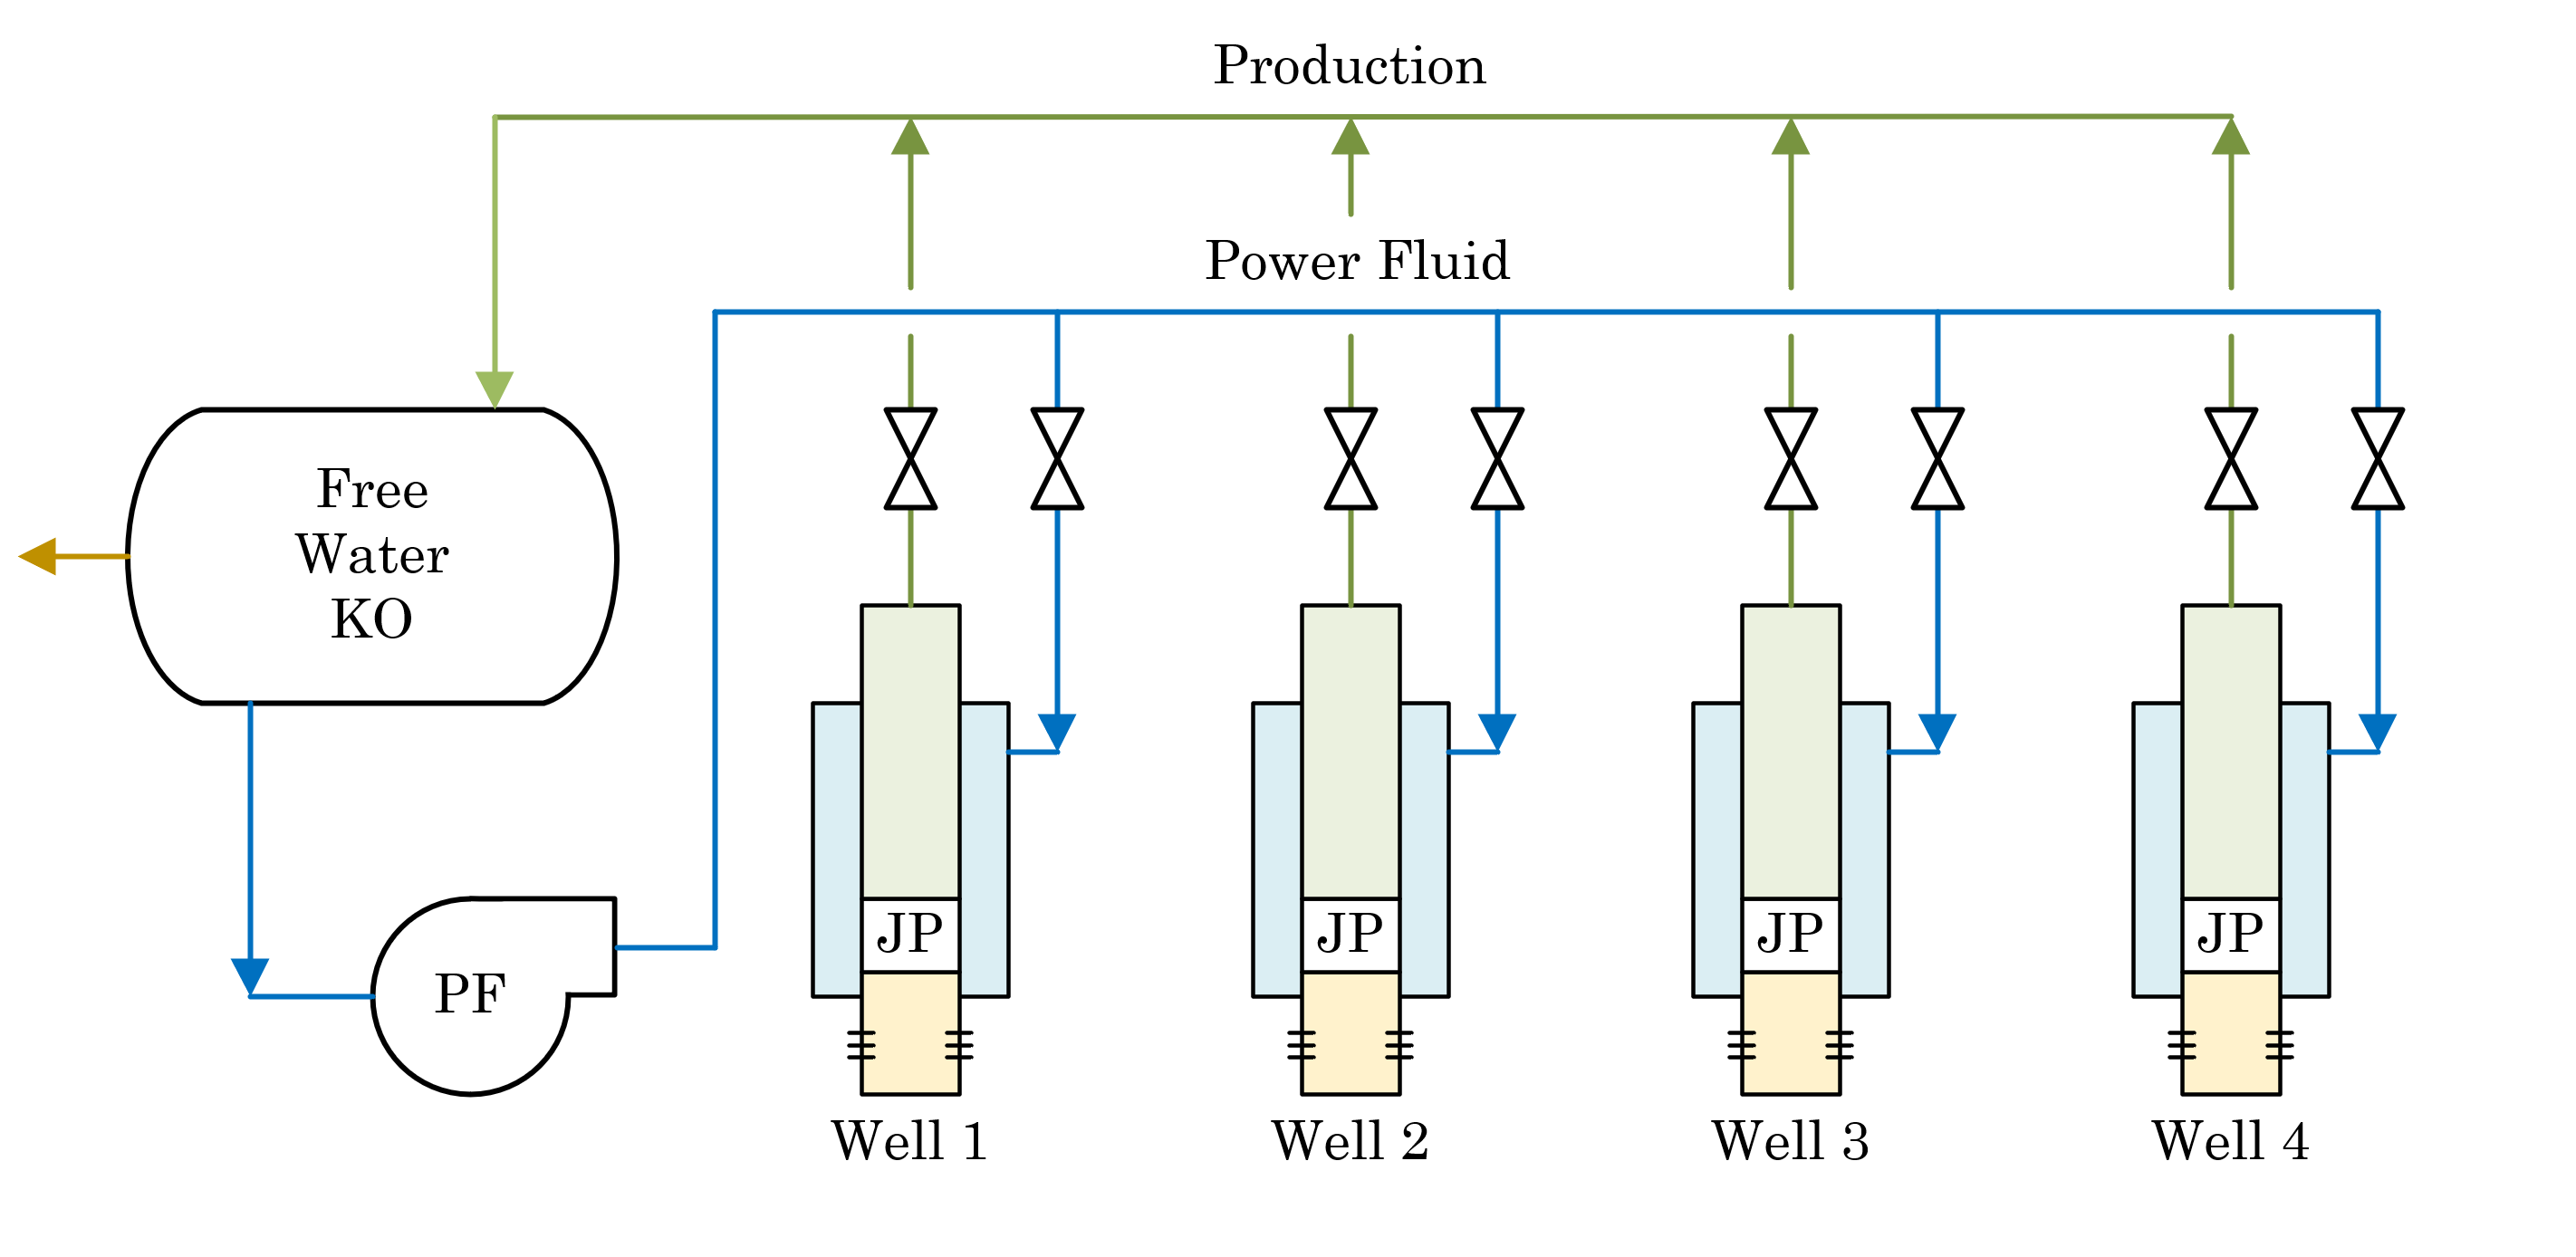
\includegraphics[width=1\linewidth]{figures/network_diagram.PNG}
    \caption{Network Diagram of Four Wells}
    \label{fig:jetpump_network}
\end{figure}

\section{Mathematical Model}

The oil production from a well on jet pump is represented with the equation below. Where $q_{oil}$ is the oil produced and $q_{pf}$ is the power fluid volume required.

\begin{equation*}
    q_{oil} = c_{1} - c_{2} \exp{(-q_{pf} c_{3})}
\end{equation*}

The coefficients $c_{1}$, $c_{2}$ and $c_{3}$ are found in a separate numerical scheme and are dependent on the specific wells water cut, formation gas oil ratio and specific subsurface geometry. The optimization objective function and constraints are as follows:

\begin{equation*}
\begin{aligned}
    \text{maximize } & \sum_{i=1}^{k} q_{\text{oil}}^{i} \\
    \text{subject to } & \sum_{i=1}^{k} q_{\text{pf}}^{i} \leq Q_{\text{pf}}^{\text{pump}} \\
    & q_{\text{pf}}^{i} \geq 0 \\
\end{aligned}
\end{equation*}

The index $i$ represents a specific unique oil well that is on the network.

\section{Optimization Schemes}

Two separate optimization schemes will be analyzed in the problem. The first scheme is the application of a quasi newton method that was applied for gas lift wells \cite{gas_lift_quasi}. The quasi newton method only requires first derivatives, where the Hessian is approximated using a positive definite matrix \cite{optm_griva}. Two quasi newton methods are currently of interest. The first method is the Broyden, Fletcher, Goldfarb and Shanno (BFGS). The second method is the Davidon, Fletcher and Powell (DFP). The exact method to apply will be selected during the project.\\

The second is the application of an equal slope method. This method relies on calculating the required oil and gas demand for each well at a series of finite points. The curves are then added together to match on the same slope / derivative. A value of gas lift is selected that ensures each well is operating at the same slope point. \cite{gas_lift_econ} This scheme is assumed to be much more computationally expensive than the quasi newtwon method.

\section{Desired Outcomes}

The following are the desired outcomes from this project.

\begin{enumerate}[i)]
    \item Apply power fluid optimization schemes with quasi newton method and equal slope method
    \item Compare the convergence and required computation for each scheme.
    \item Test accuracy in a constrained and unconstrained case.
\end{enumerate}

\printbibliography

\end{document}

